\documentclass{article}
\usepackage{graphicx} % Required for inserting images

\title{Problem Set 6}
\author{savannahjsimpson }
\date{March 12 2024}

\begin{document}

\maketitle

\section{Data Set Description and Cleaning }
\begin{itemize}
\item For the purposes of this assignment, I will be utilizing the R dataset titled "txhousing" which has 8,602 observations of the 9 following variables: city, year, month, sales, volume, median, listings, inventory, and date. While I would have liked to have worked with fewer observations, there is no fair way to differentiate which entries are more significant. Instead of cleaning the data, I manipulated certain variables to get a clean picture. 
\item As for data set significance, I chose this set as it made sense given the parameters of this assignment and correlated with my previous data. In the last problem set I focused on property values in Florida, and this was an interesting opportunity to compare circumstances across states. 
\end{itemize}

\section{Data Visualization}
\begin{itemize}
\item Firgure 1: This line plot visualizes the trend of median home prices over time in Texas. Here we can see the ultimate trend in home prices, as well as the ranges that they are maintaining over time. 
\item Figure 2: This scatter plot visualizes the relationship between sales volume and median home prices in Texas. While many of the observations overlap, it is expected given the magnitude of the dataset. Additionally, the large clusters are more appropriate considering the overall trend volumes. 
\item Figure 3: This box plot visualizes the range of home prices in the most prominent Texas counties. Focusing on the top 5 counties allowed as a way of "cleaning" out other observations while maintaining significance. Here we can see the interquartile range, median, and outlier prices for the desired counties. 
\end{itemize}

\begin{figure}[htp]
    \centering
    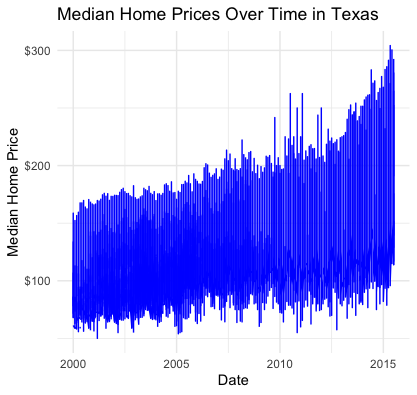
\includegraphics[width=9cm]{PS6a_Simpson.png}
\end{figure}

\begin{figure}[htp]
    \centering
    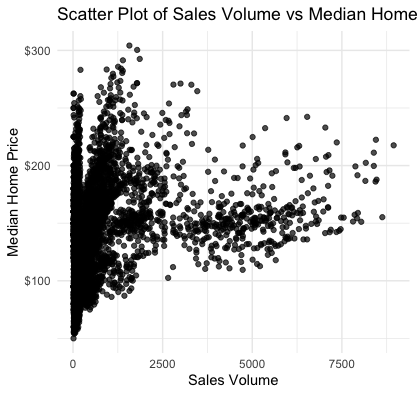
\includegraphics[width=9cm]{PS6b_Simpson.png}
\end{figure}


\begin{figure}[htp]
    \centering
    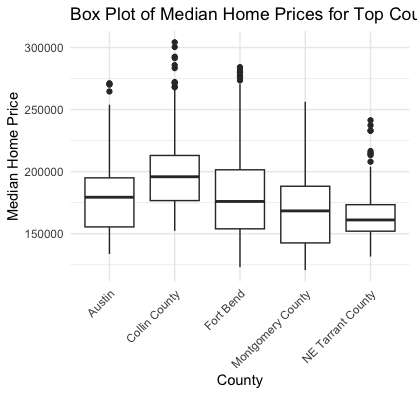
\includegraphics[width=9cm]{PS6c_Simpson.png}
\end{figure}


\end{document}
